\newgeometry{top=1in,bottom=1in,right=1in,left=1in}
\chapter*{Bilag 1: 7-bit tegnsæt}
\thispagestyle{empty}
\setcounter{page}{1}
\begin{figure}[H]
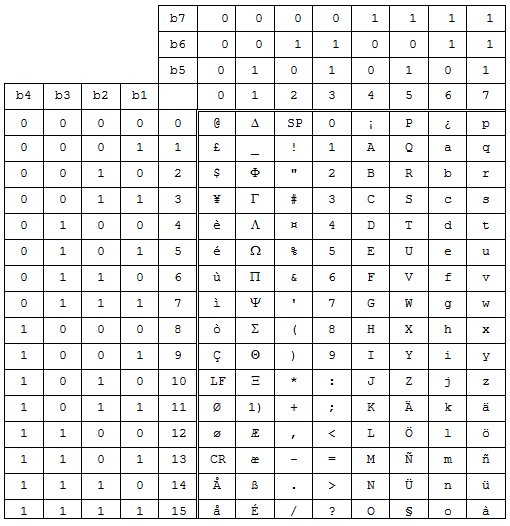
\includegraphics [width=\linewidth]{Billeder/tegnsaet.png}
\caption {Her ses skemaet for bit 7 tegnsættet. Ved 0x1b ses tegnet 1), der er et escape tegn til den ekstra tabel, som ses på figur \ref{tegnsaet2}}
\label {tegnsaet}
\end{figure}

\chapter*{Bilag 2: 7-bit tegnsæt del 2}
\thispagestyle{empty}
\setcounter{page}{1}
\begin{figure}[H]
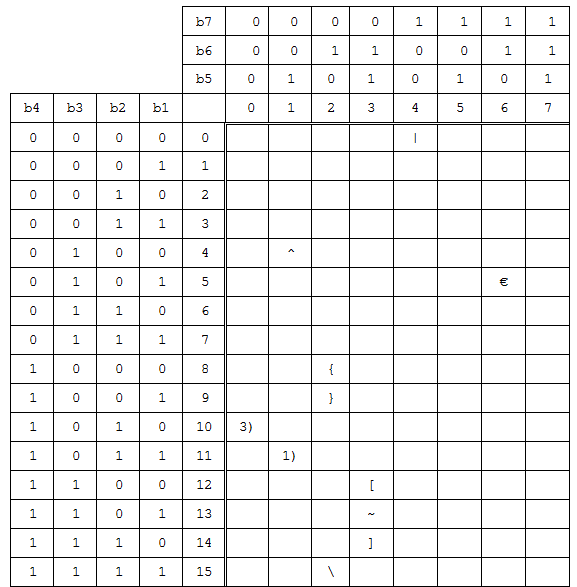
\includegraphics [width=\linewidth]{Billeder/tegnsaet2.png}
\caption {Den ekstra tabel for bit 7 tegnsaettet. Det samme tegn 1), er her et escape tegn som er reserveret hvis en ny ekstra tabel introduceres. Tegnet 3) er et form feed tegn, som er et escape tegn der starter en ny side}
\label {tegnsaet2}
\end{figure}

\chapter*{Bilag 3: Mest brugte tegn i dansk Wikipedia}
\thispagestyle{empty}
\setcounter{page}{1}
\begin{figure}[H]
\centering
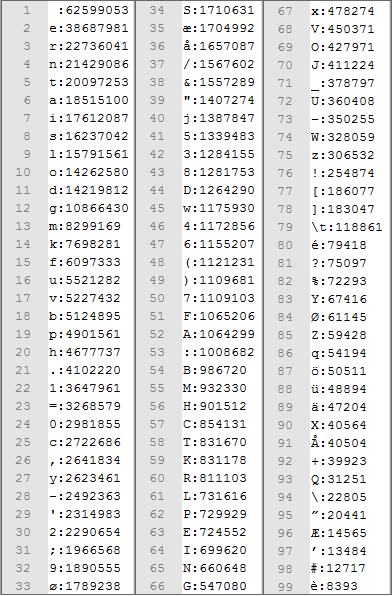
\includegraphics []{Billeder/wikiBilag.png}
\caption {Tabellen viser top 100 over mest brugte tegn i over 340.000 danske Wikipedia artikler}
\label {wikiAnalyse}
\end{figure}

\chapter*{Bilag 4: Mest brugte tegn i vores SMS-analyse}
\thispagestyle{empty}
\setcounter{page}{1}
\begin{figure}[H]
\centering
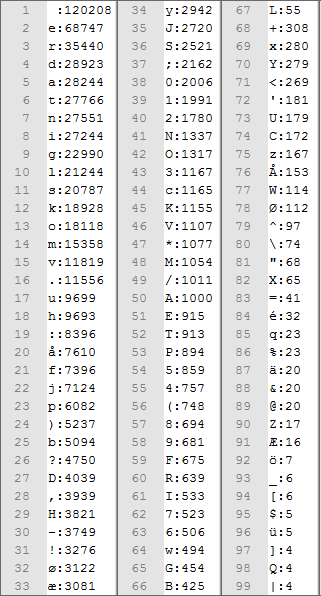
\includegraphics []{Billeder/SMSbilag.png}
\caption {Figuren viser top 100 over mest brugte tegn fra vores SMS analyse af over 13.000 SMS beskeder.}
\label {SMSanalyse}
\end{figure}
\thispagestyle{empty}

\chapter*{Bilag 5: Kildekoder}
\setcounter{page}{1}
\definecolor{gray}{rgb}{0.4,0.4,0.4}
\lstset{
  language=C,
  basicstyle=\ttfamily,
  columns=fullflexible,
  showstringspaces=false,
  commentstyle=\color{gray}\upshape,
  keywordstyle=\color{Blue},
  morestring=[b]",
  stringstyle=\color{gray}
}
\lstdefinelanguage{C}
{keywords={HuffNode}%
}

\section*{Programmet (Huffman.c)}
\lstinputlisting[language=C, morekeywords={HuffNode, uchar, BitStream}]{Program/new/Huffman.c}
\clearpage
\section*{Header (HuffmanLibrary.h)}
\lstinputlisting[language=C, morekeywords={HuffNode, uchar, BitStream}]{Program/new/HuffmanLibrary.h}


\chapter*{Bilag 6: Projektforslag}
\thispagestyle{empty}
\subsection*{Hvordan kan man konvertere et billede?}
Hvordan skal man lave et godt system til konvertering af billeder?

\subsubsection*{Problemstilling}
Nogle hjemmesider accepterer kun billeder af bestemte formater. Hvis et billede har et forkert format, afviser hjemmesiden at uploade billedet. Tilsvarende accepterer andre hjemmesider kun billeder af visse størrelser.

\subsubsection*{Formål}
Projektets formål er at udvikle en metode til konvertering af billeder, f.eks fra PNG til JPEG. Metoden skal være anvendelig på den platform, man vælger.

\subsubsection*{Mål}
Målet kan være at definere en model, som beskriver konvertering af billedfiler og at lave en implementation af en prototype, der kan udføre konverteringen.

\subsubsection*{Datalogiske emner}
Algoritmer til behandling af billedfiler, datastrukturer.

\subsubsection*{Eksempler på kontekstuelle spørgsmål og problemstillinger}
Hvem kunne have interesse i at konvertere billeder? Hvorfor accepterer nogle hjemmesider kun bestemte formater? Hvilke problemer kan en konverteringsteknologi føre med sig med hensyn til brugbarhed?

\subsubsection*{Forslagsstiller}
B228